\chapter{Additional theoretical background}
This appendix states several theoretical results from deterministic dynamical systems and stochastic calculus which are used throughout this thesis, and in particular the proofs presented in \Cref{sec:paper_proofs}.
These results are included for completeness, so we do not include proofs and instead refer the reader to other sources.

\section{Deterministic results}
The flow map satisfies the following properties, under ASSUMPTIONS?
For any \(r, s, t \in [0,T]\) and points \(x,w \in \R^n\),
\begin{enumerate}
	\item \(F_{s}^{t}\) is invertible with inverse
	      \[
		      \left[F_{s}^{t}\right]^{-1}\left(w\right) = F_{t}^{s}\left(w\right).
	      \]
	\item \(F_s^{t}\left(F_{r}^{s}(x)\right) = F_{r}^{t}\left(x\right)\)
\end{enumerate}


An important result for establishing bounds on a function given an integral inequality is Gr\"onwall's inequality.

\begin{theorem}[Gr\"onwall's inequality]\label{thm:gronwall}
	Let \(\alpha, \beta, u: [a,b] \to \R\) be functions such that \(\beta\) and \(u\) are continuous and that the negative part of \(\alpha\) is integrable on every closed and bounded subset of \([a,b]\).
	Then, if \(\beta\) is non-negative and for all \(t \in [a,b]\),
	\[
		u(t) \leq \alpha(t) + \int_a^t{\beta(\tau)u(\tau)\dif\tau}
	\]
	then
	\[
		u(t) \leq \alpha(t) + \int_a^t{\alpha(\tau)\beta(\tau)\exp\left(\int_\tau^{t}{\beta(s)\dif s}\right)\dif\tau}.
	\]
	Additionally, if \(\alpha\) is non-decreasing, then
	\[
		u(t) \leq \alpha(t) \exp\left(\int_a^t{\beta(\tau)\dif\tau}\right)
	\]
\end{theorem}
\begin{proof}
	The integral form of this result was first stated and proven by \citet{Bellman_1943_StabilitySolutionsLinear}.
\end{proof}


\section{Analytical tools for It\^o calculus}
There are several tools available for the analytic treatment of It\^o integrals and solutions to stochastic differential equations, which we make particular use of in the proofs presented in \Cref{ch:linear_theory}.
The first is It\^o's isometry, which relates the expectation of an It\^o integral to that of a deterministic one and is useful for computing moments.
\begin{theorem}[It\^o's Isometry]\label{thm:ito_isom}
	Let \(f: \Omega \times [0,T] \to \R\) be an It\^o integrable stochastic process.
	Then, for any \(t \in [0,T]\)
	\[
		\avg{\left(\int_0^t{f\left(\omega, \tau\right)\dif W_\tau}\right)^2} = \avg{\int_0^t{f\left(\omega, \tau\right)^2\dif\tau}}
	\]
\end{theorem}
\begin{proof}
	It\^o's isometry typically arises in the formal construction of the It\^o integral.
	For example, see Section 5.1 of \citet{KallianpurSundar_2014_StochasticAnalysisDiffusion}.
\end{proof}

Next, we have It\^o's Lemma (or the It\^o Formula), which is a change-of-variables formula in stochastic calculus and can be thought of as a generalisation of the chain rule from deterministic calculus.
We state and use the multidimensional form of the Lemma for solutions to It\^o stochastic differential equations, although more general forms exist (e.g. see Theorem 5.4.1 of \citet{KallianpurSundar_2014_StochasticAnalysisDiffusion}).
\begin{theorem}[It\^o's Lemma]\label{thm:ito_lemma}
	Let \(X_t\) be the strong solution to the stochastic differential equation
	\[
		\dif X_t = a\left(X_t, t\right)\dif t + b\left(X_t, t\right)\dif W_t,
	\]
	where \(a: \R^n \times [0,\infty) \to \R^n\), \(b: \R^n \times [0,\infty) \to \R^{n\times p}\) and \(W_t\) is the canonical \(p\)-dimensional Wiener process.
	If \(f: \R^n \times [0, \infty) \to \R^m\) is twice continuously-differentiable, then the stochastic process \(Y_t \coloneqq f\left(X_t, t\right)\) is a strong solution to the stochastic differential equation
	\begin{align*}
		\dif Y_t & = \left(\dpd{f}{t}\left(X_t, t\right) + \nabla f\left(X_t, t\right) a\left(X_t, t\right) + \frac12\mathrm{tr}\left[b\left(X_t, t\right)^{\T} \nabla\nabla f\left(X_t, t\right) b\left(X_t, t\right)\right] \right)\dif t \\
		         & \qquad\qquad\qquad\qquad + \nabla f\left(X_t, t\right)b\left(X_t, t\right) \dif W_t.
	\end{align*}
\end{theorem}
\begin{proof}

\end{proof}

Our third and final result is the Burkholder-Davis-Gundy inequality, which when applied to stochastic integrals provides bounds on the expected norm.
\begin{theorem}[Burkholder-Davis-Gundy Inequality]\label{thm:bdg}
	Let \(M_t\) be an It\^o-integrable stochastic process taking values in \(\R^n\).
	Then, for any \(p > 0\) there exists constants \(c_p, C_p > 0\) independent of the stochastic process \(M_t\) such that
	\[
		c_p\avg{\left(\int_0^t{\norm{M_\tau}^2\dif \tau}\right)^p} \leq \avg{\sup_{\tau \in \left[0, t\right]}\norm{\int_0^\tau{M_s\dif W_s}}^{2p}} \leq C_p\avg{\left(\int_0^t{\norm{M_\tau}^2\dif \tau}\right)^p}.
	\]
\end{theorem}
\begin{proof}
	This result is stated and proven as Theorem 5.6.3 of \citet{KallianpurSundar_2014_StochasticAnalysisDiffusion}.
\end{proof}

As with ordinary differential equations, we are interested in knowing when a given stochastic differential equation has solutions, and when those solutions are unique.
Since we are now dealing with random processes, the notion of uniqueness is no longer well-defined.

The main distinction are that strong solutions are defined on the \emph{same} probability space as the given driving Wiener process, whereas weak solutions are defined on \emph{any} probability space with a possibly different Wiener process.
This leads to two different notion of uniqueness; a strong solution \(y_t\) is strongly (or pathwise) unique if for any other strong solution \(x_t\),
\[
	P\left(y_t = x_t \, \forall t \in [0,T]\right) = 1.
\]
If \(x_t\) was not defined on the same probability space as \(y_t\), then the probability of equality would not make sense.

For our purposes, the distinction between strong and weak solutions

We can now state the requirements for the existence of unique strong solutions to \eqref{eqn:gen_sde}, in the following theorem.

\begin{theorem}[Existence and Uniqueness of SDE Solutions]\label{thm:sde_exist_unique}
	Let \(W_t\) be a standard \(m\)-dimensional Wiener process over a time interval \([0,T]\), and let \(\xi\) be a \(n\)-dimensional random vector defined on the same probability space as \(W_t\) and independent of \(W_t\).
	Consider the following stochastic differential equation evolving in \(\R^n\):
	\begin{equation}\label{eqn:sde_exist}
		\dif x_t = b\!\left(x_t, t\right)\dif t + \sigma\!\left(x_t, t\right)\dif W_t,
	\end{equation}
	subject to the initial condition \(x_0 = \xi\), with coefficients \(b\colon \R^n \times [0,T] \to \R^n\) and \(\sigma \colon \R^n \times [0,T] \to \R^{n \times m}\).
	Let \(\mathfrak{B}\!\left(A\right)\) generically denotes the Borel \(\sigma\)-algebra on the set \(A \subseteq \R^q\).
	Suppose that the coefficients \(b\) and \(\sigma\) are such that
	\begin{romanate}
		\item each component \(b_j\colon \R^n \times [0,T] \to \R^n\) of \(b\) is measurable with respect to \(\mathfrak{B}\!\left([0,T]\right) \times \mathfrak{B}\!\left(\R^n\right)\).

		\item For each \(t \in [0,T]\), the restriction \(b_j\!\left(t, \cdot\right)\) is measurable with respect to \(\mathfrak{B}\!\left(\R^n\right)\).

		\item each component \(\sigma_{ij}\colon \R^n \times [0,T] \to \R^n\) of \(\sigma\) is  \(\mathfrak{B}\!\left([0,T]\right) \times \mathfrak{B}\!\left(\R^n\right)\) measurable.

		\item For each \(t \in [0,T]\), the restriction \(\sigma_{ij}\!\left(t, \cdot\right)\) is measurable with respect to \(\mathfrak{B}\!\left(\R^n\right)\).

		\item (linear growth) there exists a constant \(K_G\) such that for all \(t \in [0,T]\) and \(x \in \R^n\),
		\[
			\norm{b\!\left(x,t\right)}^2 + \norm{\sigma\!\left(x,t\right)} \leq K_G\left(1 + \norm{x}^2\right).
		\]

		\item (Lipschitz continuity) these exists a constant \(K_L\) such that for all \(t \in [0,T]\) and \(x,y \in \R^n\),
		\[
			\norm{b\!\left(x,t\right) - b\!\left(y,t\right)}^2 + \norm{\sigma\!\left(x,t\right) - \sigma\!\left(y,t\right)}^2 \leq K_L\norm{x - y}^2.
		\]

	\end{romanate}
	Then, \eqref{eqn:sde_exist} has a unique strong solution.
\end{theorem}
\begin{proof}
	A proof is available in any standard textbook on It\^o calculus, e.g. in the proof of Theorem 6.2.1 in \citet{KallianpurSundar_2014_StochasticAnalysisDiffusion}.
\end{proof}





% \section{Aspects of stochastic parameterisation}
% When using deterministic systems to model real-world phenomena, there are many ways in which uncertainty can arise.
% For instance,

% Stochastic parameterisation is a
% These unresolved subgrid effects are accounted for by introducing stochastic noise into the otherwise deterministic model.

% \citet{BernerEtAl_2017_StochasticParameterizationNew}

% \citet{LeutbecherEtAl_2017_StochasticRepresentationsModel}

% \subsection{Additive versus multiplicative noise}

% When \(\sigma = \sigma(t)\) depends only on \(t\), then noise is considered \emph{additive}.
% If there is spatial dependence in \(\sigma\), i.e. \(\sigma = \sigma(x,t)\), then the noise considered \emph{multiplicative}.



% For instance, \citet{SuraEtAl_2005_MultiplicativeNoiseNonGaussianity} shows that the non-Gaussian statistics observed in atmospheric regimes can arise from linear models with multiplicative noise.


\section{Stochastic sensitivity}

The statistics of \(z_\epsilon\left(x,T\right)\) and \(P_\epsilon(x,\theta)\) are considered in the limit as \(\epsilon\downarrow 0\), which provides a characterisation of the uncertainty of the model \emph{independently} of the scale of the noise.
\citet{Balasuriya_2020_StochasticSensitivityComputable} provided computable expressions for the mean and variance of \(P_\epsilon\left(x,\theta\right)\) in this limit of small noise, which we summarise here.
For proofs of these results, see the appendices of \citet{Balasuriya_2020_StochasticSensitivityComputable}.

The first result established by \citet{Balasuriya_2020_StochasticSensitivityComputable} is that the expected location is deterministic, in the following sense.
\begin{theorem}[\citealt{Balasuriya_2020_StochasticSensitivityComputable}]
	For all \(x \in \R^2\),
	\[
		\lim_{\epsilon\downarrow 0}\avg{z_\epsilon(x,T)} = 0.
	\]
\end{theorem}

The variance of \(P_\epsilon\left(x,\theta\right)\) is used to assign a computable scalar measure of uncertainty to the trajectory.

\begin{definition}[\citealt{Balasuriya_2020_StochasticSensitivityComputable}]
	\begin{alpharate}
		\item The \textbf{anisotropic uncertainty} is a scalar field \(A: \R^2\times\left[-\pi/2, \pi/2\right) \to [0,\infty)\) defined by
		\[
			A(x,\theta) \coloneqq \sqrt{\lim_{\epsilon\downarrow 0}\var{P_\epsilon(x,\theta)}}.
		\]

		\item The \textbf{stochastic sensitivity} is a scalar field \(S: \R^2 \to [0,\infty)\) defined by
		\[
			S^2(x) \coloneqq \lim_{\epsilon\downarrow 0}\sup_{\theta}{\var{P_\epsilon(x,\theta)}}.
		\]
	\end{alpharate}
\end{definition}

By employing techniques from both deterministic and stochastic calculus (i.e. Gr\"onwall's inequality, the Burkholder-Davis-Gundy inequality, It\^o's Lemma), Balasuriya further established expressions for both the anisotropic uncertainty and the stochastic sensitivity that are computable given only the flow map and velocity data.

\begin{theorem}[\citealt{Balasuriya_2020_StochasticSensitivityComputable}]\label{thm:orig_s2_calculation}
	For \(x \in \R^2\), set \(w \coloneqq F_0^t(x)\).
	Then, for any \(\theta \in \left[-\pi/2, \pi/2\right)\),
	\[
		A(x,\theta) = \left(\int_0^T{\norm{\Lambda\left(x, t, T\right)J\hat{n}(\theta)}\dif t}\right)^{1/2},
	\]
	where
	\[
		\Lambda\left(x,t,T\right) \coloneqq e^{\int_t^T{\left[\nabla \cdot u\right]\left(F_0^\xi(x), \xi\right)\dif\xi}}\sigma\left(F_0^t(x), t\right)^{\T}J \nabla_w F_T^t\left(w\right),
	\]
	with the gradients \(\nabla_w\) of the flow map taken with respect to the mapped position \(w\), and
	\[
		J \coloneqq \begin{bmatrix}
			0 & -1 \\
			1 & 0
		\end{bmatrix}
	\]
	Additionally, stochastic sensitivity is computed as
	\[
		S^2(x) = P(x) + N(x),
	\]
	with
	\begin{align*}
		L(x) & \coloneqq \frac12\sum_{i=1}^2\int_0^T\left[\Lambda_{i2}\left(x,t, T\right)^2 - \Lambda_{i1}\left(x,t,T\right)^2\right]\dif t \\
		M(x) & \coloneqq \sum_{i=1}^2\int_0^T{\Lambda_{i1}\left(x,t,T\right)\Lambda_{i2}\left(x,t,T\right)\dif t}                           \\
		N(x) & \coloneqq \sqrt{L^2(x) + M^2(x)}                                                                                             \\
		P(x) & \coloneqq \abs{\frac12\sum_{i=1}^2\sum_{j=1}^2{\int_0^T{\Lambda_{ij}\left(x,t,T\right)^2\dif t}}},
	\end{align*}
	where \(\Lambda_{ij}\) is the \((i,j)\)-element of \(\Lambda\).
\end{theorem}



Accordingly, \citet{Balasuriya_2020_StochasticSensitivityComputable} defines the \emph{resolution-scaled stochastic sensitivity} as
\begin{equation}
	S_r\left(x\right) \coloneqq \ln\left(\frac{\sqrt{S^2(x)}}{L_r}\right),
	\label{eqn:Sr_defn}
\end{equation}
where \(L_r\) is a specified spatial resolution lengthscale.
The \emph{noise-scaled stochastic sensitivity} is defined as
\begin{equation}
	S_n\left(x\right) \coloneqq \epsilon\sqrt{S^2(x)}.
	\label{eqn:Sn_defn}
\end{equation}


% \begin{figure}
% 	\begin{center}
% 		\begin{subfigure}{0.8\textwidth}
% 			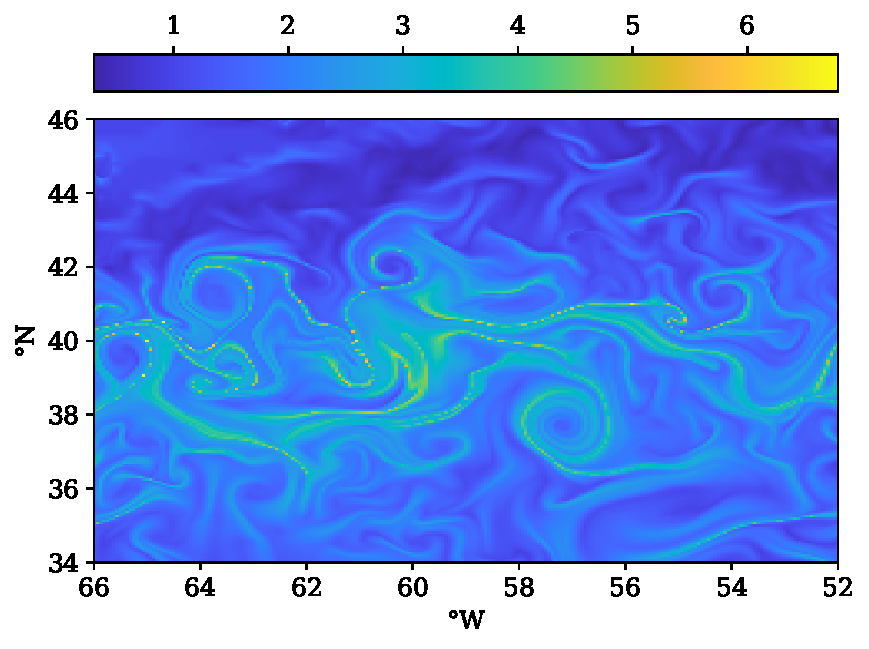
\includegraphics[width=\textwidth]{chp02_background/figures/res_scaled_stoch_sens_high_res.pdf}
% 			\caption{The resolution-scaled stochastic sensitivity field, plotted on a \(1/16\) degree resolution grid of initial conditions.}
% 			\label{fig:s2_na_ex_field}
% 		\end{subfigure}
% 		\begin{subfigure}{0.8\textwidth}
% 			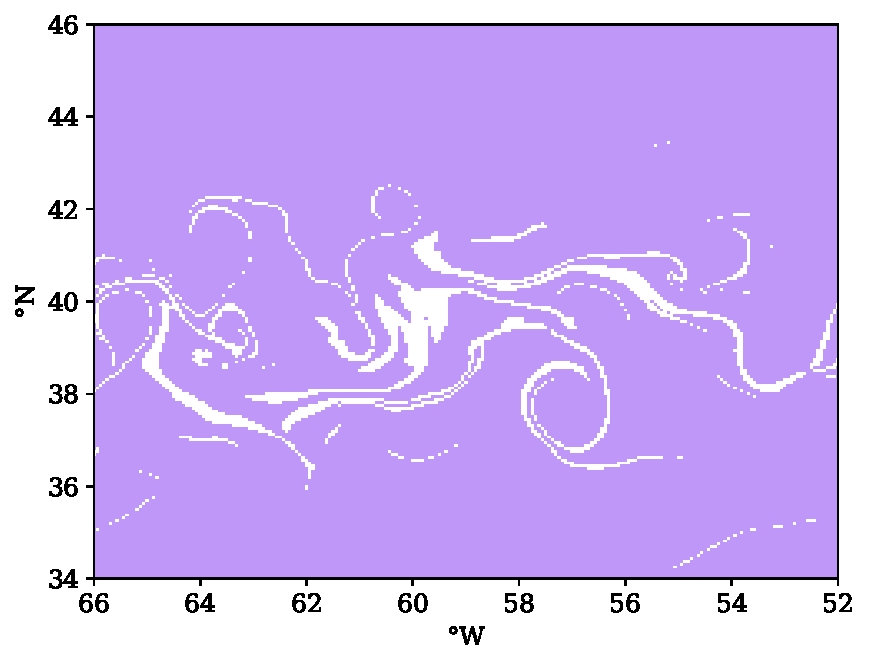
\includegraphics[width=\textwidth]{chp02_background/figures/robust_3.0_high_res.pdf}
% 			\caption{Robust sets (in purple) extracted from the stochastic sensitivity field in (a), using a lengthscale threshold of \(6\) degrees}
% 			\label{fig:s2_na_ex_sets}
% 		\end{subfigure}
% 		\caption{}
% 		\label{fig:fig:s2_na_ex}
% 	\end{center}
% \end{figure}



% Stochastic sensitivity has also provided a novel approach to extracting Lagrangian coherent structures, which are regions of a fluid that remain ``coherent'' as the flow evolves over time \citep{BalasuriyaEtAl_2018_GeneralizedLagrangianCoherent,AllshousePeacock_2015_LagrangianBasedMethods,HadjighasemEtAl_2017_CriticalComparisonLagrangian}.

% \Cref{fig:s2_na_ex_field} plots the resolution-scaled stochastic sensitivity field for a region of the North Atlantic ocean, including the Gulf Stream, as an illustrative example of how stochastic sensitivity is able to capture structures within a given flow.

% % \begin{definition}[\citealt{Balasuriya_2020_StochasticSensitivityComputable}] \label{def:ss_res_scaled}
% % 	Given a spatial resolution \(L_r\), the \emph{resolution-scaled stochastic sensitivity} is defined on \(\Omega\)
% % 	\[
% % 		S_r(x) \coloneqq \ln\left(\frac{\sqrt{S^2(x)}}{L_r}\right).
% % 	\]
% % \end{definition}
